\documentclass{standalone}

\usepackage{circuitikz}

\begin{document}
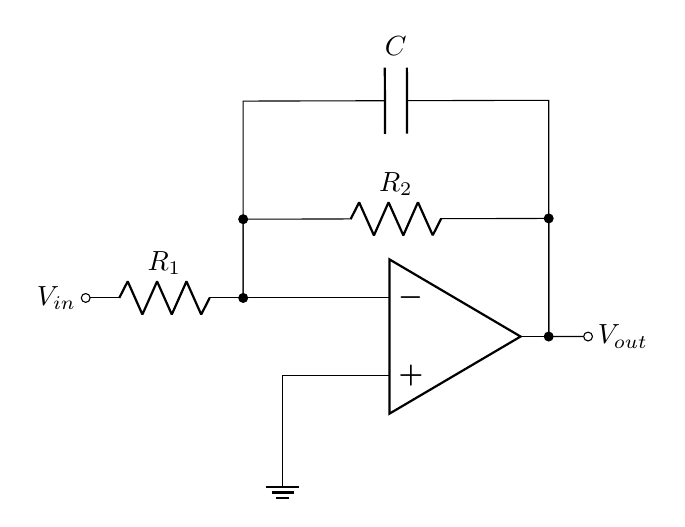
\begin{tikzpicture}
	\node[op amp, yscale=1] (opamp) at (-4,-0.5) {};
	\draw ($(opamp.-)+(-3.5,0)$) node[left] {$V_{in}$} 
	to[R, l=$R_1$, o-*] ($(opamp.-)+(-1.5,0)$) node (nodebetween1) {}
	to[short] (opamp.-);
	\draw (nodebetween1.center) to[short] ($(nodebetween1)+(0,+1)$) 
	to[R, l=$R_2$, *-*] ($(opamp.out)+(0,+1.5)$) 
	to[short] (opamp.out);
    \draw (nodebetween1.center) to[short] ($(nodebetween1)+(0,+2.5)$) 
    to[C, l=$C$]  ($(opamp.out)+(0,+3)$)
    to[short] (opamp.out);
    \draw ($(opamp.+)$) to ($(opamp.+)+(-1,0)$) to ($(opamp.+)+(-1,-1)$) node [ground] {};
    \draw (opamp.out) to[short, *-o]  ($(opamp.out)+(0.5,0)$) node[right] {$V_{out}$};
\end{tikzpicture}
\end{document}